\documentclass[12pt]{article}

\usepackage[T1]{fontenc}
\usepackage[utf8]{inputenc}
\usepackage[russian]{babel}

% page margin
\usepackage[top=2cm, bottom=2cm, left=2cm, right=2cm]{geometry}

% AMS packages
\usepackage{amsmath}
\usepackage{amssymb}
\usepackage{amsfonts}
\usepackage{amsthm}

\usepackage{float}
\usepackage{graphicx}
\usepackage{tabularx}

\usepackage{multirow}

\newcommand{\lb}{\left(}
\newcommand{\rb}{\right)}

\makeatletter
\setlength{\@fptop}{0pt}
\makeatother

\usepackage{array}
\newcolumntype{C}[1]{>{\centering\let\newline\\\arraybackslash\hspace{0pt}}m{#1}}

\begin{document} 

\begin{titlepage}
\centering
\textbf{\large Московский государственный университет имени М.В.\,Ломоносова\\
\vspace*{0.1cm} Химический факультет\\
\vspace*{0.1cm}
\noindent\makebox[\linewidth]{\rule{\paperwidth}{0.4pt}}
\vspace*{0.1cm}
 Кафедра физической химии}
\vspace*{2cm}

\begin{center}
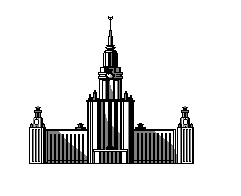
\includegraphics[width=0.3\textwidth]{pictures/logo.jpg}
\end{center}

\vspace*{2cm}
\Large \textbf{Сканирующая электронная микроскопия в режиме низкого вакуума} 
\vspace*{6cm}

\begin{flushright}
\large Работа выполнена студентом 515 группы\\
Финенко А.А.\\
\end{flushright}
\vfill
\large\textbf{Москва\\ 2017}
\end{titlepage}

\subsection*{Результаты эксперимента}

\begin{figure}[H]
	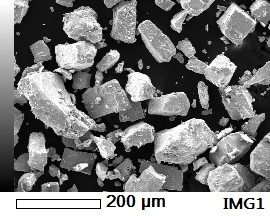
\includegraphics[width = 0.45\linewidth]{./pictures/map1_IMG1.jpg} \hspace{1em}% 
	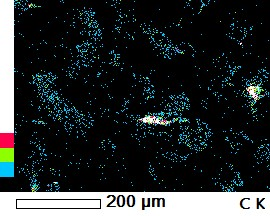
\includegraphics[width = 0.45\linewidth]{./pictures/map1_C_K.jpg} \hspace{1em}%  
	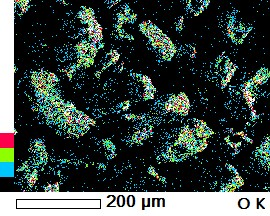
\includegraphics[width = 0.45\linewidth]{./pictures/map1_O_K.jpg} \hspace{1em}% 
	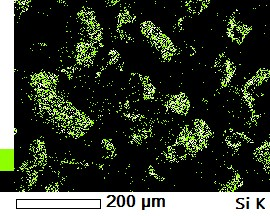
\includegraphics[width = 0.45\linewidth]{./pictures/map1_Si_K.jpg} \hspace{1em}%
	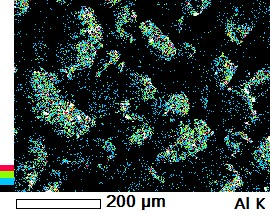
\includegraphics[width = 0.45\linewidth]{./pictures/map1_Al_K.jpg}\hspace{4.2em}%
	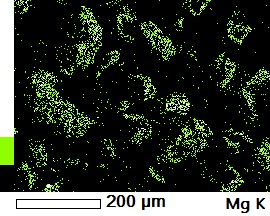
\includegraphics[width = 0.45\linewidth]{./pictures/map1_Mg_K.jpg} \hspace{1em}%
\end{figure}

\begin{figure}[H]
	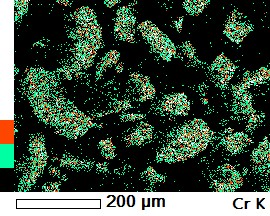
\includegraphics[width = 0.45\linewidth]{./pictures/map1_Cr_K.jpg} \hspace{1em}%
	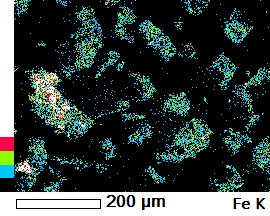
\includegraphics[width = 0.45\linewidth]{./pictures/map1_Fe_K.jpg} \hspace{1em}%
	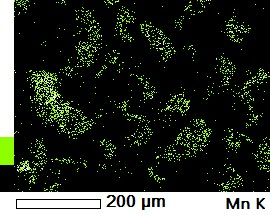
\includegraphics[width = 0.45\linewidth]{./pictures/map1_Mn_K.jpg} \hspace{4.2em}% 
	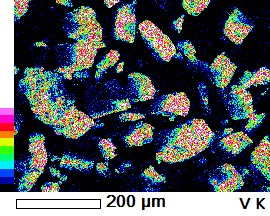
\includegraphics[width = 0.45\linewidth]{./pictures/map1_V_K.jpg} \hspace{1em}%
\end{figure}

Судя по карте распределений элементов, самым распространенным элементов является ванадий. Ванадий равномерно распределен по частицам. Помимо ванадия в частицах присутствуют магний, крмений, алюминий, хром, железо, магний и кислород. В качестве примесного элемента присутствует углерод. 

\begin{figure}[H]
	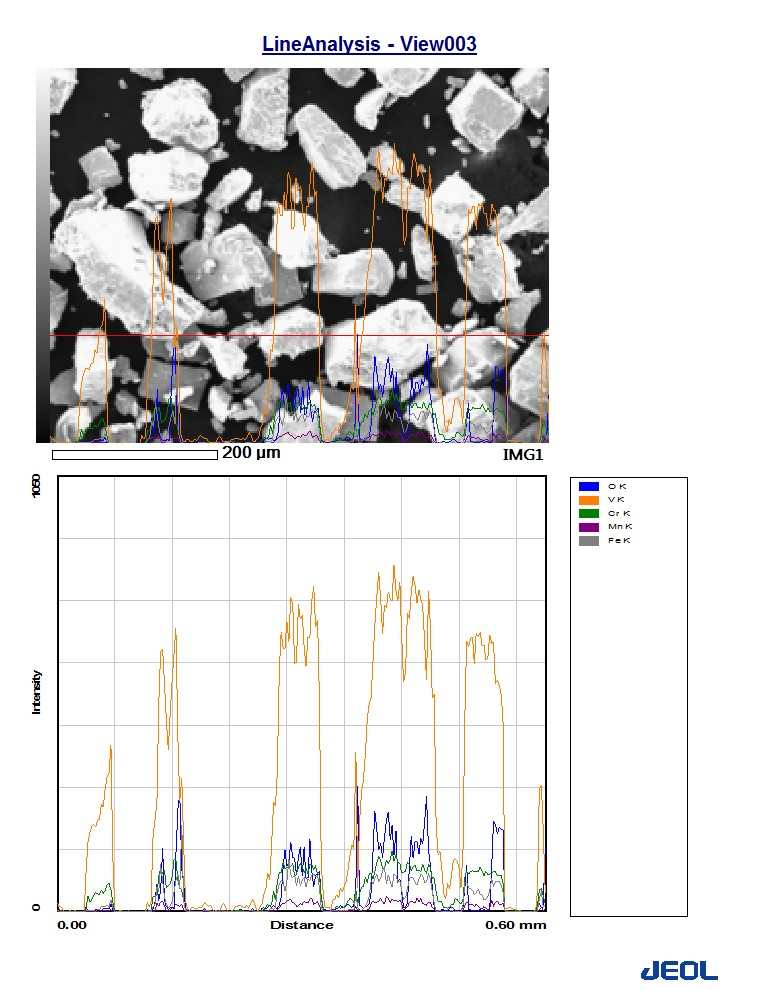
\includegraphics[width = 0.9\linewidth]{./pictures/line_spec_1.jpg}
\end{figure}
\begin{figure}[H]
	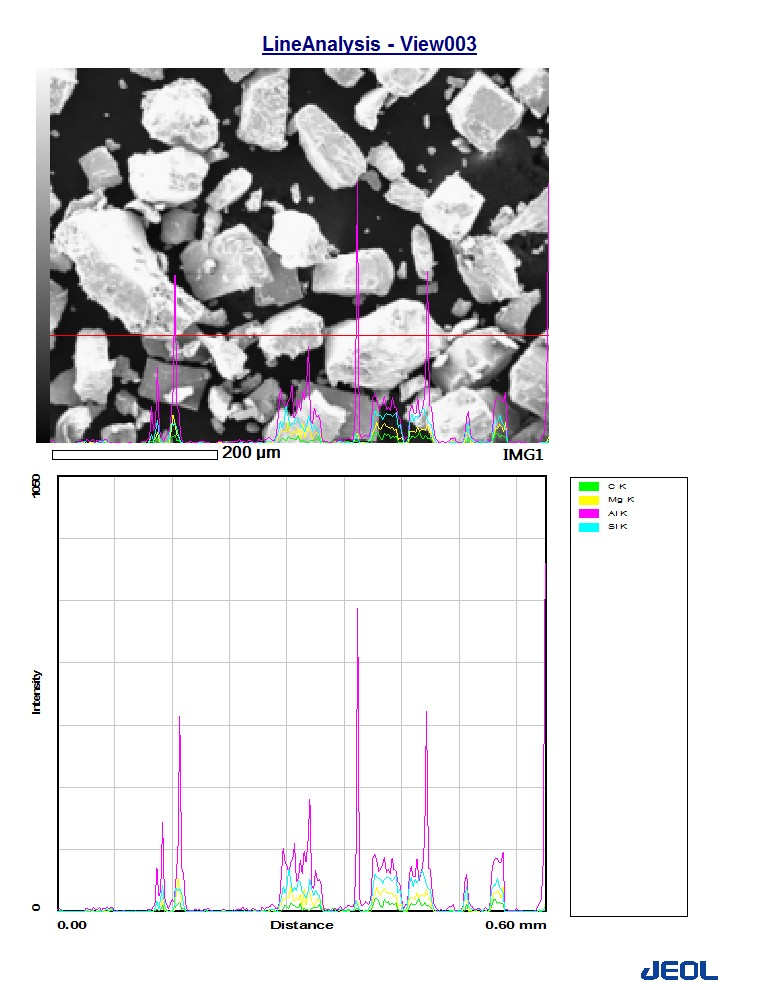
\includegraphics[width = 0.9\linewidth]{./pictures/line_spec_2.jpg}
\end{figure}

Линейное распределение элементов показывает, что основу частиц составляют металлы ванадий, хром, железо и марганец. Сигнал алюминия идет как от частиц, так и от материала подложки.

\begin{figure}[H]
	\includegraphics[width = \linewidth]{./pictures/dot_spec_1.jpg}
\end{figure}

\begin{figure}[H]
	\includegraphics[width = \linewidth]{./pictures/dot_spec_2.jpg}
\end{figure}

\begin{figure}[H]
	\includegraphics[width = \linewidth]{./pictures/dot_spec_3.jpg}
\end{figure}

\begin{figure}[H]
	\includegraphics[width = \linewidth]{./pictures/dot_spec_4.jpg}
\end{figure}

\begin{figure}[H]
	\includegraphics[width = \linewidth]{./pictures/dot_spec_5.jpg}
\end{figure}

\begin{figure}[H]
	\includegraphics[width = \linewidth]{./pictures/dot_spec_6.jpg}
\end{figure}

\begin{figure}[H]
	\includegraphics[width = \linewidth]{./pictures/dot_spec_7.jpg}
\end{figure}

\begin{figure}[H]
	\includegraphics[width = \linewidth]{./pictures/dot_spec_8.jpg}
\end{figure}

\begin{figure}[H]
	\includegraphics[width = \linewidth]{./pictures/dot_spec_9.jpg}
\end{figure}

\begin{figure}[H]
	\includegraphics[width = \linewidth]{./pictures/dot_spec_10.jpg}
\end{figure}

\begin{figure}[H]
	\includegraphics[width = \linewidth]{./pictures/area_spec.jpg}
\end{figure}

\begin{table}
	\centering
	\begin{tabular}{|c|c|c|c|c|c|}
		\hline
		Point & V, \% & Cr, \% & Fe, \% & Mn, \% & Al, \% \\
		\hline
		1 & 75.87 & 0.92 & 13.03 & 1.57 & 2.97 \\
		2 & 71.29 & 0.72 & 12.02 & 1.47 & 3.52 \\
		3 & 68.19 & 0.84 & 11.73 & 1.46 & 3.55 \\
		4 & 90.68 & 2.31 & 3.55 & 0.07 & 1.13 \\
		5 & 78.25 & 1.18 & 12.03 & 1.19 & 3.52 \\
		6 & 75.65 & 0.67 & 12.54 & 1.35 & 3.50 \\
		7 & 76.41 & 4.50 & 3.20 & 0.20 & 5.08 \\
		8 & 82.06 & 2.36 & 1.59 & - & 2.61 \\
		9 & 54.66 & 0.76 & 6.74 & 0.57 & 5.69 \\
		10 & 82.91 & 2.69 & 8.85 & 0.43 & 2.13 \\
		area & 60.42 & 0.99 & 8.15 & 0.75 & 5.054 \\ \hline
		mean & 73.85 & 1.63 & 8.5 & 0.91 & 3.52 \\ \hline
		$\sigma$ & 11.84 & 1.15 & 3.98 & 0.53 & 1.29 \\ \hline
	\end{tabular}
\end{table}

\end{document}

